\documentclass{article}

\usepackage{fancyhdr}
\usepackage{extramarks}
\usepackage{amsmath}
\usepackage{amsthm}
\usepackage{amsfonts}
\usepackage{tikz}
\usepackage[plain]{algorithm}
\usepackage{algpseudocode}
\usepackage{enumerate}
\usepackage{tikz}
\usepackage{graphicx}
\usepackage{subfigure}

\newcommand{\subsubsubsection}[1]{\paragraph{#1}\mbox{}\\}
\setcounter{secnumdepth}{4} % how many sectioning levels to assign numbers to
\setcounter{tocdepth}{4} % how many sectioning levels to show in ToC


%
% Basic Document Settings
%  

\topmargin=-0.45in
\evensidemargin=0in
\oddsidemargin=0in
\textwidth=6.5in
\textheight=9.0in
\headsep=0.25in

\linespread{1.1}

\pagestyle{fancy}


\renewcommand\headrulewidth{0.4pt}
\renewcommand\footrulewidth{0.4pt}

\setlength\parindent{0pt}


%
% Title Page
%

\title{
    \vspace{2in}
    {\large{\textbf{Report for Control System Class Projects}}}\\
    \textmd{\textbf{The Active Suspension System}}\\
    \vspace{2in}
}

\author{
	Name: \textbf{ZhuYuxuan DaiLiangtao} \\
	Student ID: 2020531016 2020531028}
\date{\today}


\everymath{\displaystyle}
\begin{document}

\maketitle
\pagebreak

\section{Introduction}

An active suspension system is a type of vehicle suspension system that uses sensors 
and actuators to continuously adjust the suspension to changing road conditions and driving situations. 
The goal of an active suspension system is to improve the ride and handling of a vehicle by increasing stability, 
reducing body roll, and reducing tire wear.\\

In an active suspension system, 
sensors detect the movements and forces acting on the vehicle, 
such as the body roll, pitch, and acceleration. 
These sensors send this information to a control unit, 
which calculates the appropriate suspension settings based on the driving conditions. 
Actuators, such as hydraulic or pneumatic cylinders, then adjust the suspension to these settings in real-time.\\

Active suspension systems are typically found on high-performance vehicles, 
as they offer greater control and adjustability compared to traditional passive suspension systems. 
However, they also tend to be more complex and expensive to maintain.\\

\subsection{Advantages}

There are several potential advantages to using an active suspension system:

\begin{enumerate}
    \item Improved ride and handling: Active suspension systems can continuously adjust the suspension to changing road conditions and driving situations, which can result in a smoother, more comfortable ride. They can also improve stability and reduce body roll, which can enhance the handling and performance of a vehicle.
    
    \item Increased tire life: By continuously adjusting the suspension to optimize tire contact with the road, active suspension systems can help to reduce tire wear and extend tire life.
    
    \item Enhanced stability: Active suspension systems can improve the stability of a vehicle by continuously adjusting the suspension to maintain optimal tire contact with the road and reduce body roll. This can be particularly useful in high-performance vehicles or in situations where stability is important, such as when driving in adverse weather conditions.
    
    \item Increased safety: By improving ride comfort and stability, active suspension systems can enhance the safety of a vehicle and reduce the risk of accidents.
    
    \item Customization: Active suspension systems offer greater adjustability than traditional passive suspension systems, which allows drivers to customize the suspension settings to their preference or to optimize for different driving situations.
\end{enumerate}

\subsection{Disadvantages}

There are several potential disadvantages to using an active suspension system:

\begin{enumerate}
    \item Cost: Active suspension systems tend to be more expensive to manufacture and maintain than traditional passive suspension systems. This can make them less appealing for use in budget-conscious vehicles.

    \item Complexity: Active suspension systems require a large number of sensors, actuators, and a control unit, which can add complexity to the design and maintenance of a vehicle.
    
    \item Reliability: As active suspension systems rely on electronic components and control algorithms, they may be more prone to failure than traditional passive suspension systems.
    
    \item Weight: The additional components required for an active suspension system can add weight to a vehicle, which can have negative impacts on fuel efficiency and performance.
    
    \item Limited adjustability: While active suspension systems offer greater adjustability than passive systems, they are still limited in their ability to adjust to a wide range of driving conditions and preferences.
\end{enumerate}

\subsection{Why a high damping ratio should be avoided}

It is generally not desirable to set a high damping coefficient in an active suspension system 
because it can lead to a harsh, uncomfortable ride. 
The damping coefficient, or damping ratio, 
determines the amount of damping, or resistance, 
in a suspension system. 
A high damping coefficient means that the suspension is more resistant to movement, 
which can result in a firmer, stiffer ride.\\

In an active suspension system, 
the goal is typically to provide a smooth, 
comfortable ride while also maintaining good stability and handling. 
To achieve this, the damping coefficient is typically set to a moderate level 
that provides sufficient damping to control body movements and maintain tire contact with the road, 
but not so much that the ride becomes uncomfortable.\\

It is worth noting that the optimal damping coefficient for a given suspension system will depend on various factors, 
such as the type and weight of the vehicle, the type of suspension, 
and the driving conditions. 
In some cases, 
it may be appropriate to set a higher damping coefficient for certain driving situations, 
such as when driving on rough or uneven roads. 
However, in general, it is best to avoid setting a damping coefficient that is too high in an active suspension system.\\

\section{System Modeling}

\subsection{Suspension System}

\begin{figure}[htbp]
    \centering
    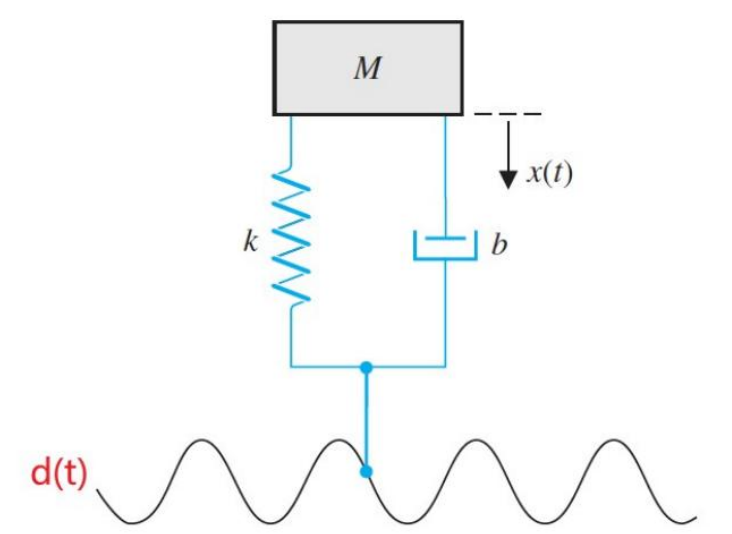
\includegraphics[width=0.5\textwidth]{1.jpg}
    \caption{Simplified automobile suspension system}
\end{figure}

The main part of the system we want to control is shown in Figure 1.
The system is a simplified automobile suspension system, which consists of a spring, a damper, and a mass.
The spring and the damper are connected in parallel, and the mass is the symbol for a automobile.
Then we define the following parameters:\\

\begin{itemize}
    \item $M$: mass of the automobile
    \item $k$: spring constant
    \item $b$: damping coefficient
    \item $x$: displacement of the automobile
    \item $d$: input of ground fluctuation to the system
\end{itemize}

By Newton's second law, we can get the following equation where gravity is offset by the supporting force of the tyres.
\begin{equation*}
    M\ddot{x}+b\dot{x}+kx=b\dot{d}+kd
\end{equation*}\\

Assume the initial condition is $x(0)=0$ and $\dot{x}(0)=0$, we can get the following solution by taking Laplace transform at both sides of the equation:
\begin{equation*}
    \frac{X(s)}{D(s)}=\frac{bs+k}{Ms^2+bs+k}
\end{equation*}\\

From the given parameters as $M=1kg,\ b=4N\cdot s/m,\ k=18N/m$, we can get the following transfer function:
\begin{equation*}
    \frac{X(s)}{D(s)}=\frac{4s+18}{s^2+4s+18}
\end{equation*}\\

And with the help from matlab, we can sketch the Bode diagram of the system as shown in Figure 2:\\

\begin{figure}[htbp]
    \centering
    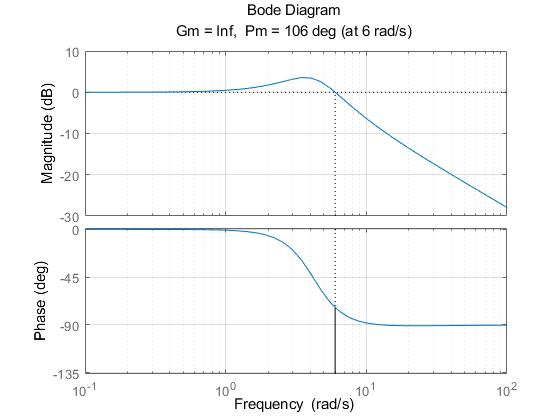
\includegraphics[width=0.5\textwidth]{2.jpg}
    \caption{Block diagram of the system}
\end{figure}

Moreover, we can notice that it is a feedback system,
and its corresponding block diagram can be built in the simulink as shown below.\\

\begin{figure}[htbp]
    \centering
    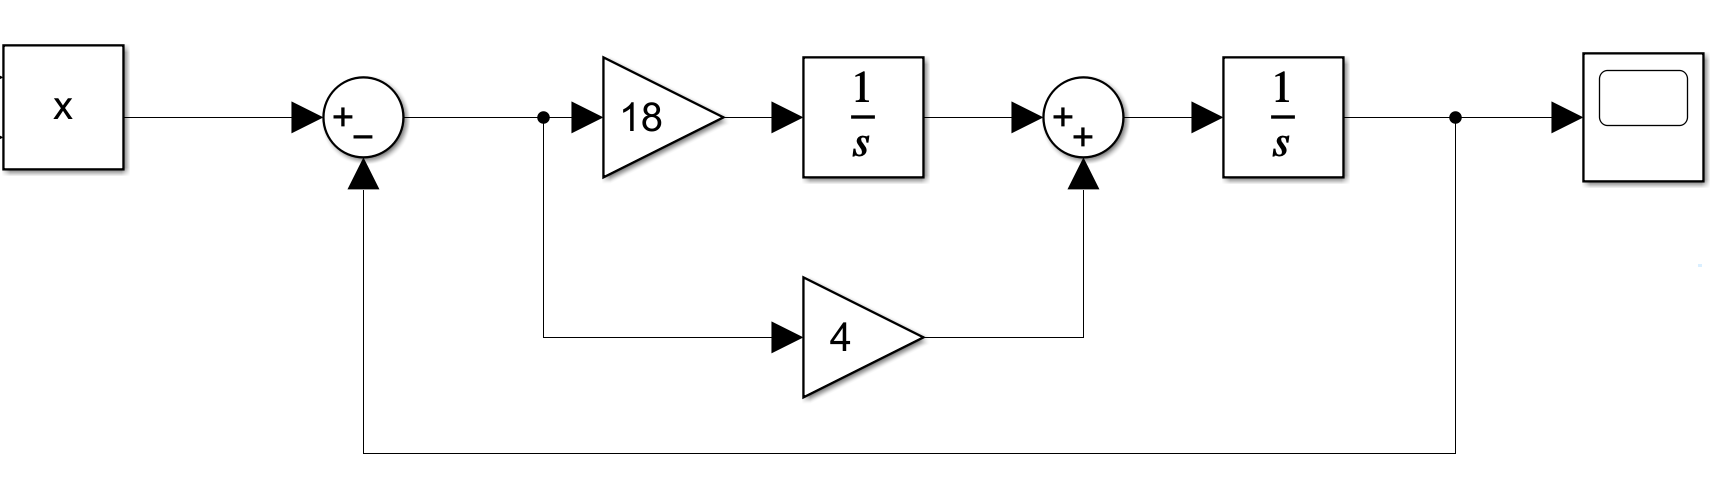
\includegraphics[width=0.5\textwidth]{3.jpg}
    \caption{Bode diagram of the system}
\end{figure}

\subsection{Damper System}

One of the beneficial applications of an automotive control system is the active control of the suspension system. 
One feedback control system uses a shock absorber consisting of a cylinder filled with a compressible fluid that provides both spring and damping forces. 
The cylinder has a plunger activated by a gear motor,
a displacement-measuring sensor, and a piston. 
Spring force is generated by piston displacement, 
which compresses the fluid. During piston displacement, 
the pressure imbalance across the piston is used to control damping. 
The plunger varies the internal volume of the cylinder.
The system is shown in Figure 3.\\

\begin{figure}[htbp]
    \centering
    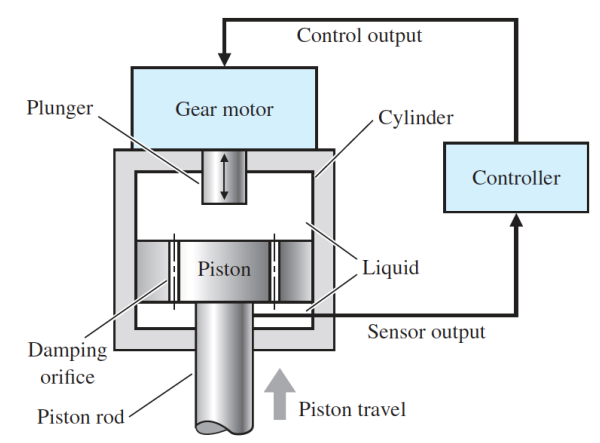
\includegraphics[width=0.5\textwidth]{4.jpg}
    \caption{Damper system}
\end{figure}

To be more simplified, we can transform the physical system into a block diagram as shown in Figure 4.\\

\begin{figure}[htbp]
    \centering
    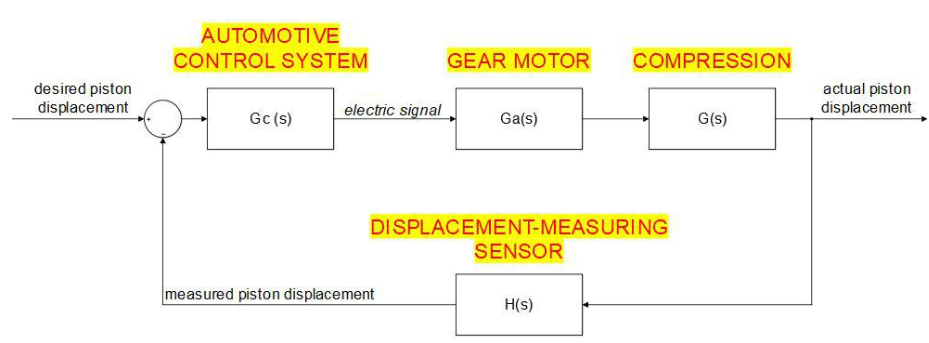
\includegraphics[width=0.5\textwidth]{5.jpg}
    \caption{Block diagram of the damper system}
\end{figure}

Due to the requirement of Question 2, we can further simplify the system as shown in Figure 5.\\

\begin{figure}[htbp]
    \centering
    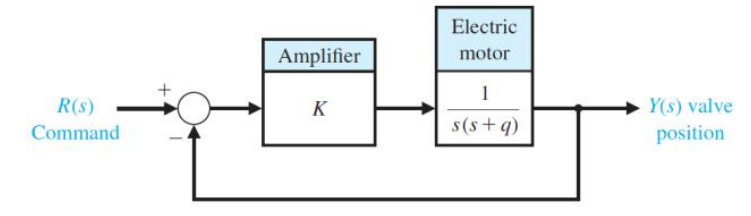
\includegraphics[width=0.5\textwidth]{6.jpg}
    \caption{Simplified block diagram of the damper system}
\end{figure}

Therefore, we can directly get the corresponding transfer function:
\begin{equation*}
    T(s)=\frac{Y(s)}{R(s)}=\frac{K}{s^2+qs+K}
\end{equation*}\\

The performance of the system can be selected as the settling time $T_s\leq 0.1s$ (with a 2\% criterion).
To obtain the required settling time, we can rewrite the transfer function as:
\begin{equation*}
    T(s)=\frac{w_n^2}{s^2+2\zeta w_ns+w_n^2}
\end{equation*}\\

Compared the three criterions for a second order system as shown in figure,
we find that the ITAE criterion is the most suitable one for this system.\\

\begin{figure}
    \centering
    \subfigure[ISE]{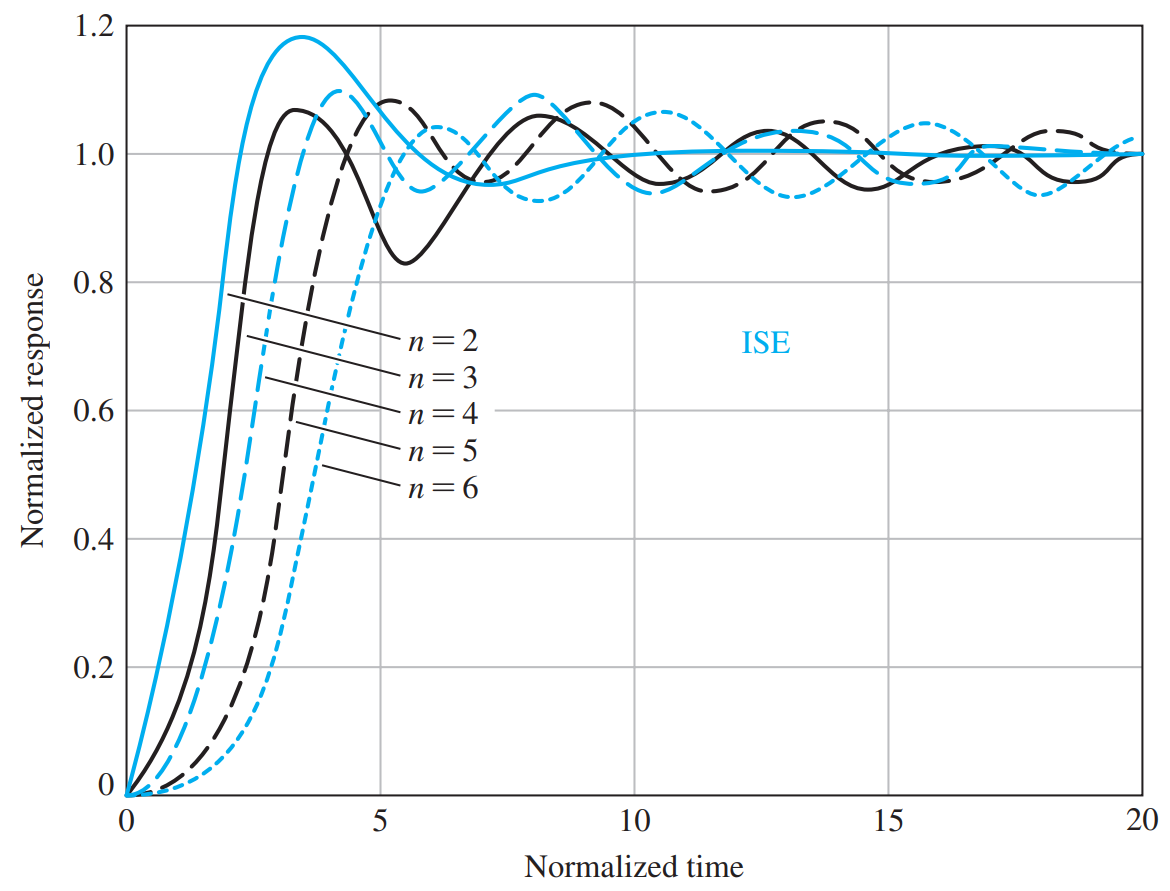
\includegraphics[width=0.3\textwidth]{7.1.jpg}}
    \subfigure[IAE]{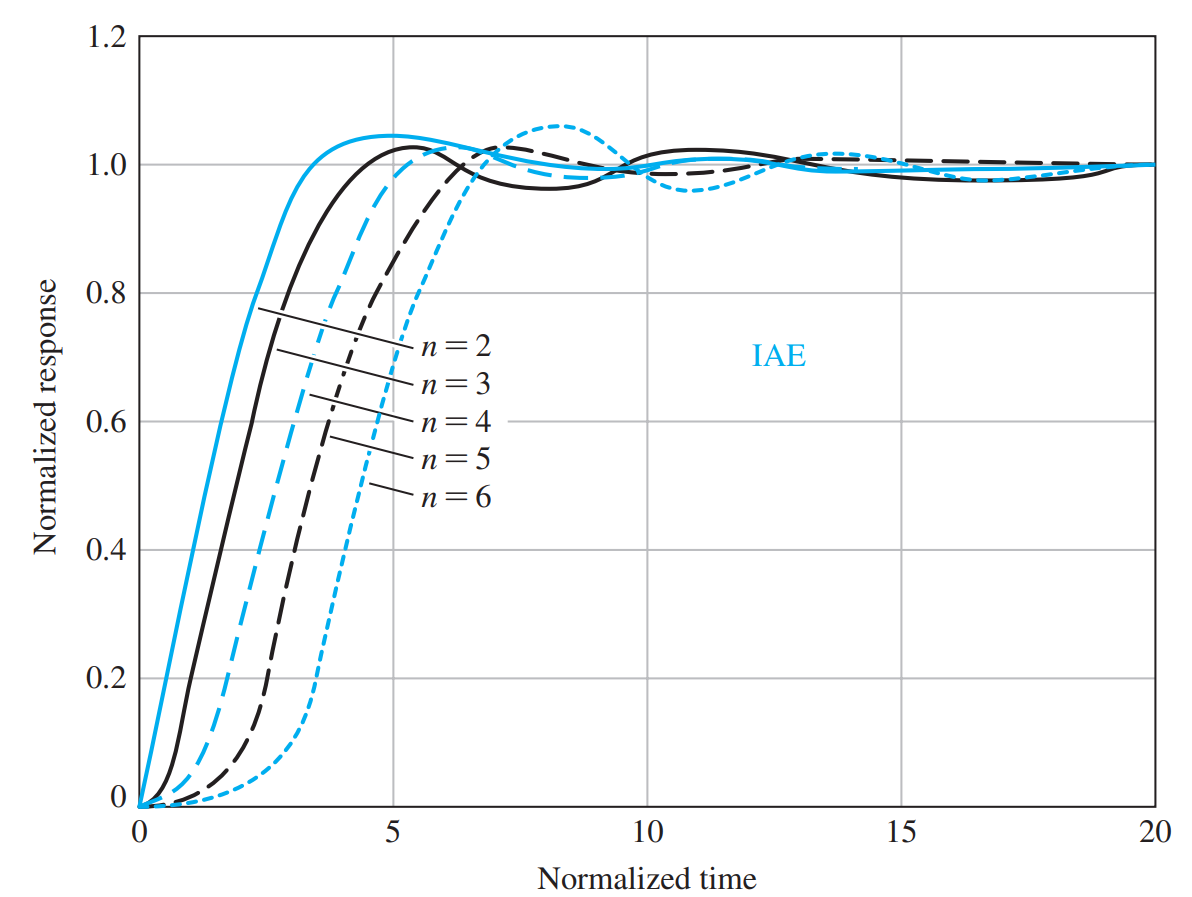
\includegraphics[width=0.3\textwidth]{7.2.jpg}}
    \subfigure[ITAE]{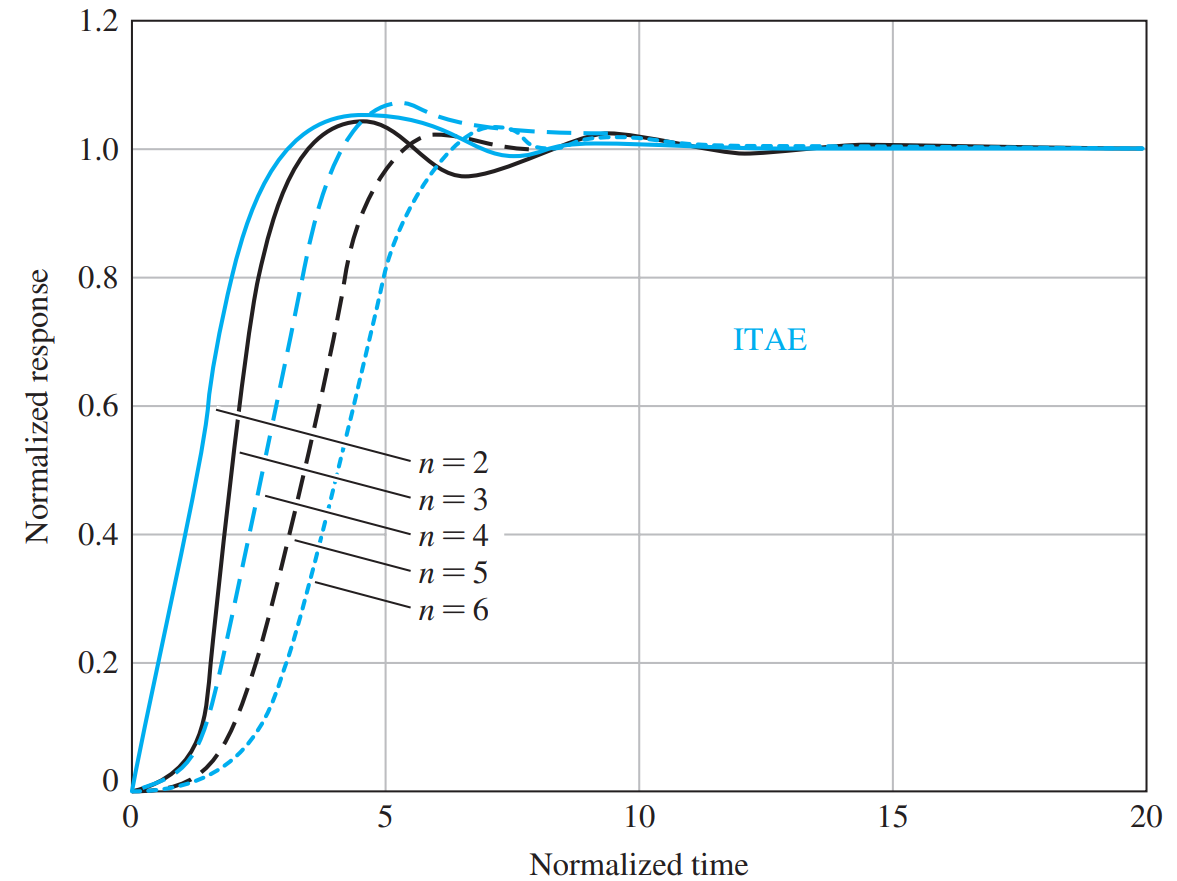
\includegraphics[width=0.3\textwidth]{7.3.jpg}}
    \caption{Step Response of different criterions}
\end{figure}

Therefore, from Table 5.3 in the textbook, we obtain that
\begin{align*}
    2\zeta w_n&=1.4w_n\\
    \Rightarrow \zeta&=0.7
\end{align*}\\

Then, with the requirement for $T_s<=0.1s$, we can get the following equation:
\begin{align*}
    \frac{4}{\zeta w_n} &\leq 0.1\\
    \Rightarrow w_n\geq \frac{40}{0.7}&=57.14
\end{align*}\\

To maintain a certain margin, we can select $w_n=60$.
Then, we can get the following transfer function:
\begin{equation*}
    T(s)=\frac{60^2}{s^2+2\cdot 0.7\cdot 60s+60^2}
\end{equation*}\\

Thus, the required parameters are
\begin{align*}
    K&=3600\\
    q&=84
\end{align*}\\

The estimated percentage overshoot can be calculated as:
\begin{align*}
    P.O.&=100e^{-\frac{\pi \zeta}{\sqrt{1-\zeta ^2}}}\\
    &\approx 4.5\%
\end{align*}\\

To verify the estimation, we can use the matlab to sketch the step response of the feedback system as shown in Figure 6.
The largest overshoot is 4.598\%, and the settling time is $T_s = 0.1s$ as labeled in the figure, which is consistent with the estimation.\\

\begin{figure}[htbp]
    \centering
    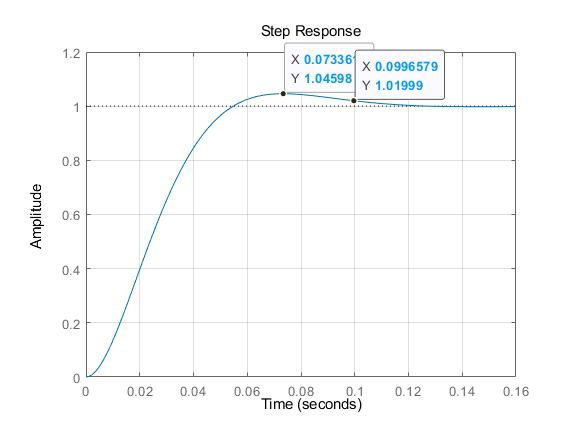
\includegraphics[width=0.5\textwidth]{8.jpg}
    \caption{Step response of the damper system}
\end{figure}

\section{Control Law for damping ratio}
As we mentioned in the Section 1.3,
the damping ratio should be selected among a moderate region.
If the damping ratio is too high or too low, 
the active suspension system can not work operately.\\

\subsection{Preparation}

Therefore, we use the root locus to determine the range of $b$ at first.\\
Rewrite the characteristic equation as 
\begin{equation*}
    1+b\cdot \frac{s}{Ms^2+k}=1+b\cdot \frac{s}{s^2+18}=0
\end{equation*}

Then the root locus can be shown in Figure 9.\\

\begin{figure}[htbp]
    \centering
    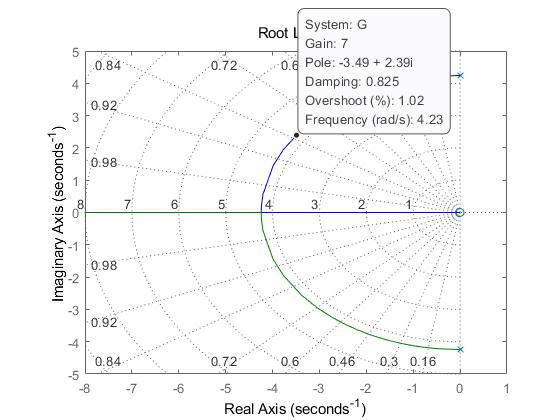
\includegraphics[width=0.5\textwidth]{9.jpg}
    \caption{Root locus of the characteristic equation}
\end{figure}

From the root locus,
we can verify that no matter how large $\zeta$ is,
the system is always stable.\\

Before we consider a sinusoidal input,
we can first consider a step input to check some more properties of the system.
This method is feasible because a sinusoidal input can be approximated by a series of step inputs.
Using the value of $b$ in the previous section, the step response of the system is shown in Figure 10.\\

\begin{figure}[htbp]
    \centering
    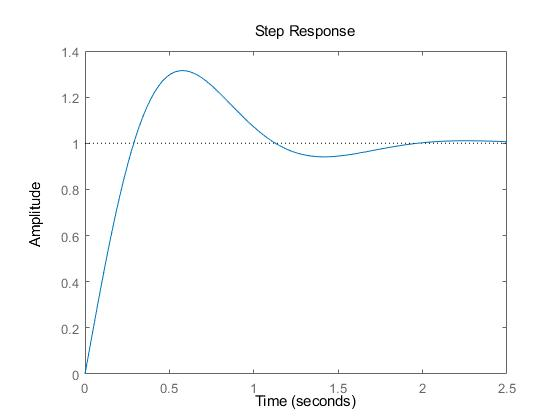
\includegraphics[width=0.5\textwidth]{10.jpg}
    \caption{Step response of the system}
\end{figure}

Such system does not have some properties that we want, for example,
the system has a large overshoot and a long settling time.\\

If we want to reduce the overshoot and the settling time at the same time,
we can determine the exact value of $b$ by using the root locus.
However, $b$ need to be modified according to the input signal, as well as the speed.
Therefore, we can first optimize one of the two indexes to get a limitation of $b$.\\

To determine which index to optimize, we can consider our riding experience in reality.
When we are driving a car, we can feel the vibration of the car body.
We would rather bear a larger vibration than a longer bump.
So we select $T_s\leq 1.15s $ here.
Then, we can get the following equation:
\begin{align*}
    \frac{4}{\zeta w_n} &\leq 0.5\\
    w_n &\approx \sqrt{18}\approx 4.24\\
    \Rightarrow b&\geq 7
\end{align*}
the corresponding point is labeled in Figure 9.\\

In additon, the lower limit we calculate here uses a lot of approximation,
so the exact value is not important.
The most valuable imformation we obtain is that $b$ should not be too small.
Although, in section 1.3, we have already discussed the disadvantage of a large $b$,
the task does not require us to consider the trade-off between the performance and the other cost.
Therefore, we can select a large $b$ to reduce the overshoot and the settling time at certain speed.\\

\subsection{The effect of speed}

Since the problem assumes that the the input of the ground is sinusoidal,
the faster the speed is, the higher the frequency of the input is.
Then we can simply assume the input is $d(t) = sin(vt)*u(t)$,
where $v$ is the speed of the car.
Here, we can assume the input as a one-side signal because a limit number of bumps appear on the road.
Then the input signal will only occurs during a certain time period.\\

The Laplace transform of the input signal is
\begin{equation*}
    D(s)=\mathbf{L} \{d(t)\}=\frac{v}{s^2+v^2}
\end{equation*}\\

Then the output of the system is
\begin{equation*}
    X(s) = \frac{v(bs+k)}{(s^2+v^2)(s^2+bs+k)}
\end{equation*}\\

The output in the time domain can be obtained by matlab, and the result is
\begin{align*}
    \begin{array}{l}
        \frac{324\,\sin \left(t\,v\right)-18\,v^2 \,\sin \left(t\,v\right)-b\,v^3 \,\cos \left(t\,v\right)+b^2 \,v^2 \,\sin \left(t\,v\right)}{\sigma_1 }+\frac{b\,v^3 \,{\mathrm{e}}^{-\frac{b\,t}{2}} \,{\left(\cosh \left(t\,\sigma_2 \right)-\frac{\sinh \left(t\,\sigma_2 \right)\,{\left(\frac{b}{2}+\frac{324\,v-18\,v^3 }{b\,v^3 }\right)}}{\sigma_2 }\right)}}{\sigma_1 }\\
        \mathrm{}\\
        \textrm{where}\\
        \mathrm{}\\
        \;\;\sigma_1 =b^2 \,v^2 +v^4 -36\,v^2 +324\\
        \mathrm{}\\
        \;\;\sigma_2 =\sqrt{\frac{b^2 }{4}-18}
        \end{array}
\end{align*}\\

From the time domain expression, we find that $b$ and $v$ appear as a product,
which points out that a large $v$ need a small $b$, and vice versa.\\

\subsection{Attemption result}

As we discussed before, we select the low limit of $b$ as 5.
With the help of simulink, we test a few couples of $b$ and $v$.
Before the result is displayed, we need to explain our select requirements.\\

Given the amplitude of the input signal, for a relatively high speed,
the gain of the system can be smaller than 1 for a correctly chosen $b$.
Therefore, the best $b$ we choose for a high speed is the one that can make the gain as small as possible,
on the basis of not breaking the low limit of $b$.\\

For a relatively low speed, the smallest gain of the system can be around 1 for a large $b$.
Therefore, the best $b$ we choose for a low speed is the smallest one that can make the gain equals to 1.
Here, we fully consider the disadvantages of a large $b$, and try our best to avoid it.\\

\begin{figure}[htbp]
    \centering
    \subfigure[$v=30m/s,b=5$]{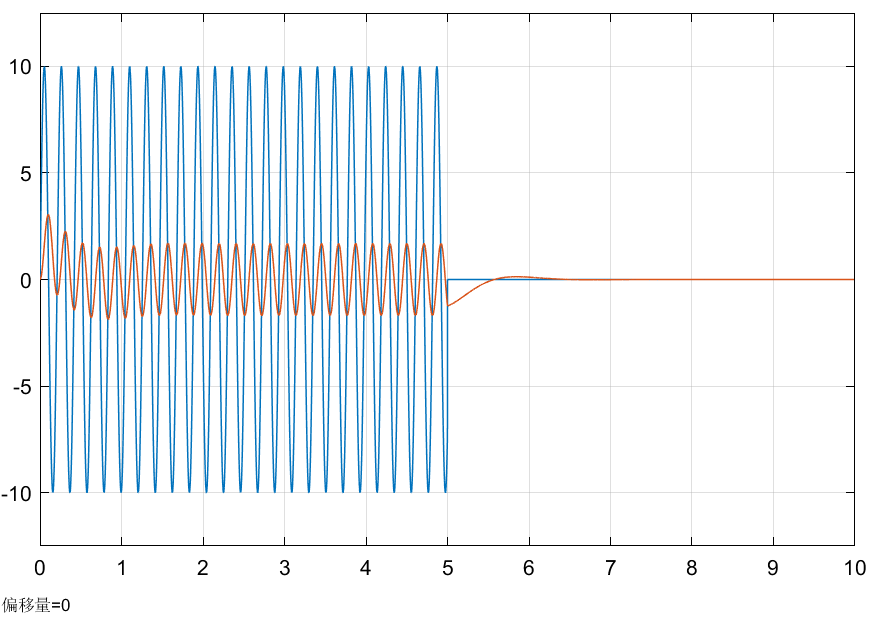
\includegraphics[width=0.3\textwidth]{11.1.jpg}}
    \subfigure[$v=20m/s,b=5$]{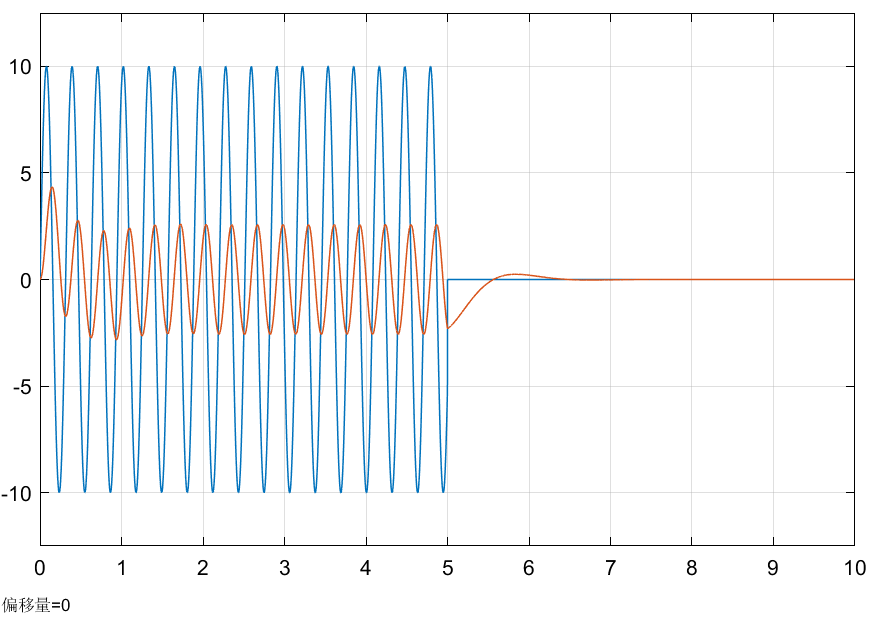
\includegraphics[width=0.3\textwidth]{11.2.jpg}}
    \subfigure[$v=10m/s,b=5$]{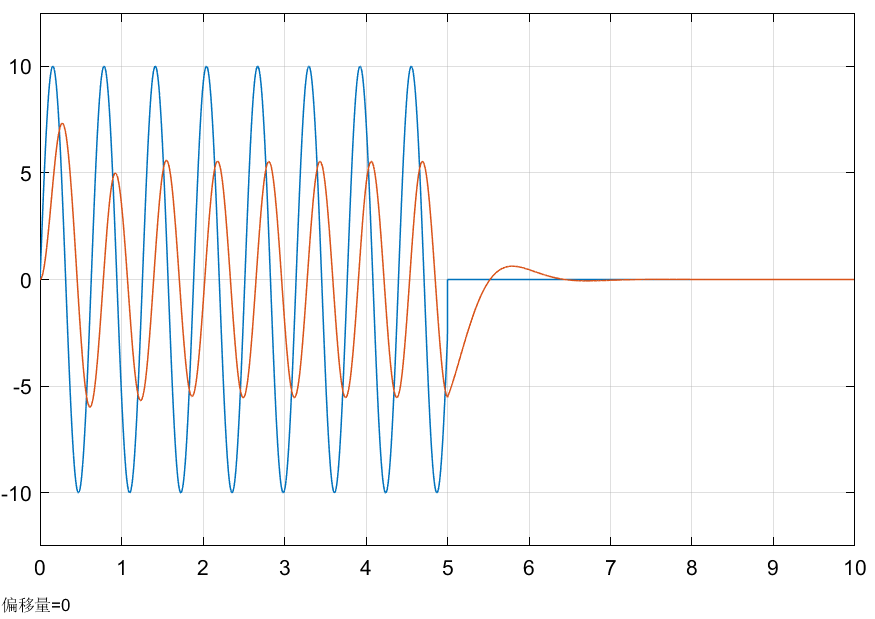
\includegraphics[width=0.3\textwidth]{11.3.jpg}}
    \caption{High speed simulation result} 
\end{figure}

\begin{figure}[htbp]
    \centering
    \subfigure[$v=5m/s,b=30$]{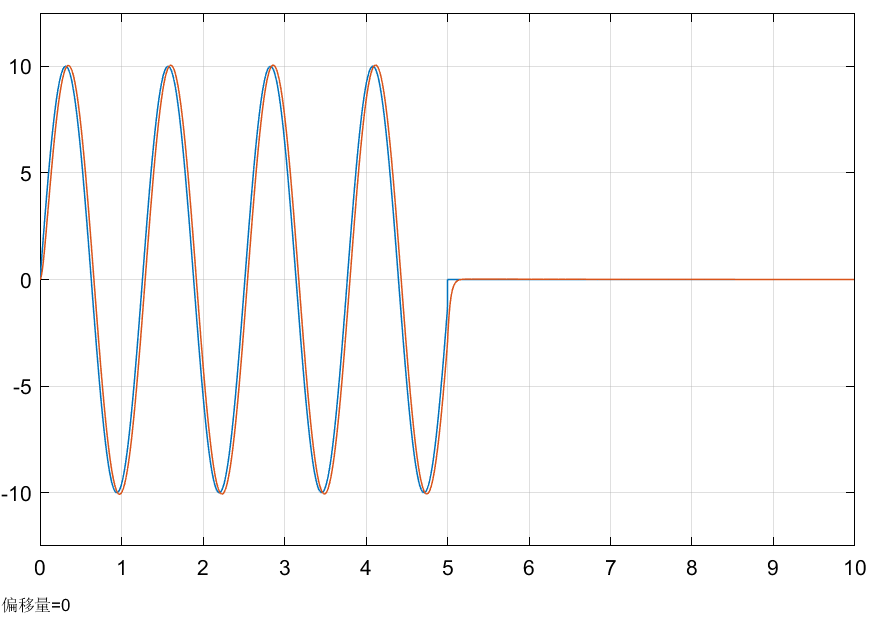
\includegraphics[width=0.3\textwidth]{11.4.jpg}}
    \subfigure[$v=3m/s,b=40$]{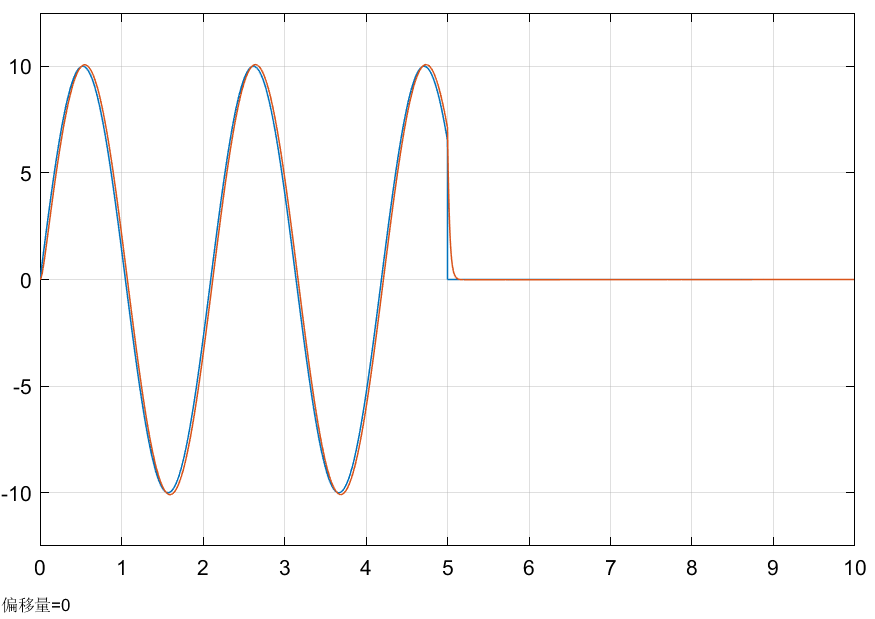
\includegraphics[width=0.3\textwidth]{11.5.jpg}}
    \subfigure[$v=1m/s,b=50$]{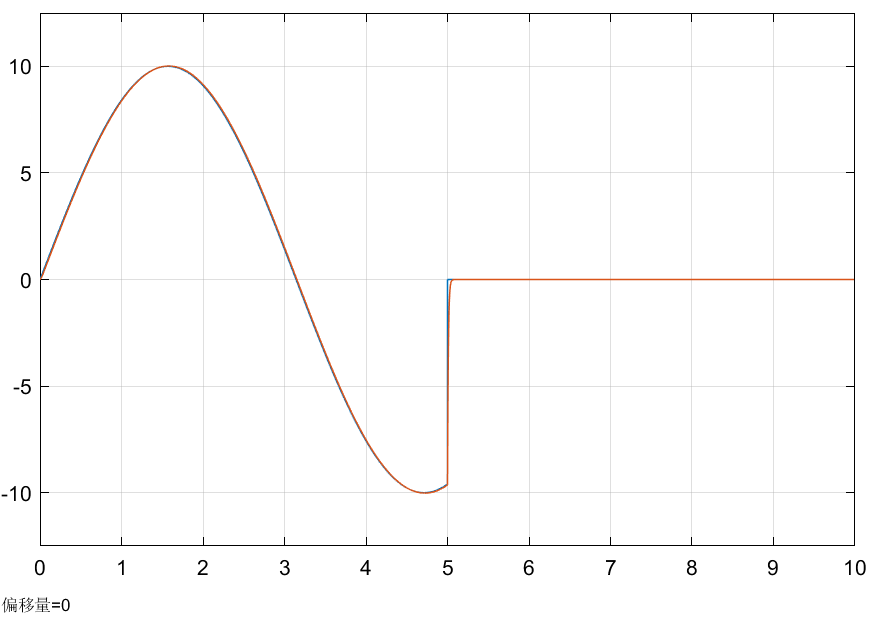
\includegraphics[width=0.3\textwidth]{11.6.jpg}}
    \caption{Low speed simulation result}
\end{figure}

From the simulation result, we can see that our optimal category to choose $b$ is
\begin{itemize}
    \item For a high speed, $b=5$.
    \item For a low speed, $b$ linear increases with the speed.
\end{itemize}

\subsection{Control design}

Following the optimal category we discussed before, we can obtain the relationship between $b$ and $v$
as shown in the following figure.\\

\begin{figure}[htbp]
    \centering
    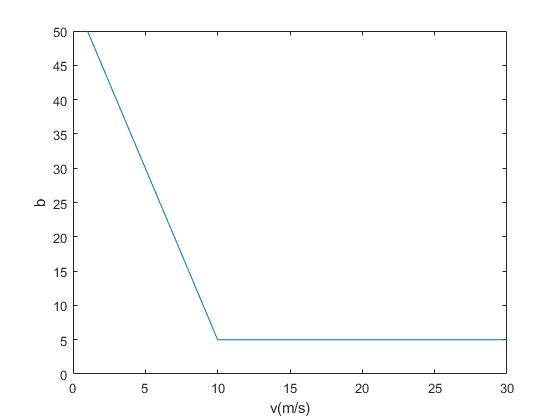
\includegraphics[width=0.5\textwidth]{13.jpg}
    \caption{Relationship between $b$ and $v$}
\end{figure}

Then, if the system has a speed sensor,
we can simply design a digital controller to control the $b$ according to the relationship above.\\


\subsubsection{Analog speed observer design}

Unfortunately, the system may not have the sensor to obtain the speed of the car.
So we try to design a analog observer to estimate the speed of the car from the input signal $d(t)$.\\

It is difficult to design a such observer in the way of the whole textbook,
since $v$ appears at both the numerator and the denominator of $D(s)$.
Therefore, we consider another way to achieve the same goal.
Consider the derivative of the input signal in time domain:
\begin{align*}
    \frac{d }{d t}d(t) &=v\cos(vt)\\
    \frac{d^2}{d x^2} d(t) &=-v^2\sin(vt)\\
    \int d(t) \,dx &= -\frac{1}{v}\cos(vt)
\end{align*}\\

With the knowledge of the analog circuit,
we know the divider can be bulit based on the analog circuit completely without any digital sampling.
Moreover, it is also practical to use circuits to implement the integrator and the differentiator.
Therefore, we can obtain the speed of the car by
\begin{equation*}
    \frac{\frac{d }{d t}d(t)}{\int d(t) \,dx} = -v^2
\end{equation*}\\

Or in another way:
\begin{equation*}
    \frac{\frac{d^2}{d x^2} d(t)}{d(t)}=-v^2
\end{equation*}

However, it is queit difficult to realize the root opening operation in the analog circuit.
Therefore, we use a quadratic equation to approximate relationship between $b$ and $v$.
Using a piecewise function as 
\begin{align*}
    b(v) = \begin{cases}
        5, & v\geq 10\\
        \frac{50}{99}v^2+\frac{5495}{99}, & 0<v<10
    \end{cases}
\end{align*}\\

And the corresponding curve is
\begin{figure}[htbp]
    \centering
    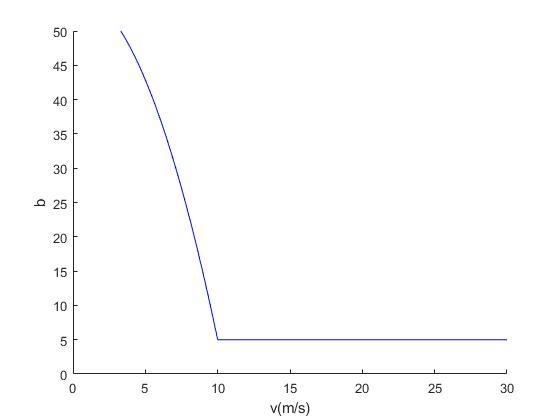
\includegraphics[width=0.5\textwidth]{14.jpg}
    \caption{Relationship between $b$ and $v$}
\end{figure}

One may wander that why we can select the value of $b$ as 5 when $v\geq 10$.
This is practical in analog circuit by using a comparator or adjusting the supply voltage of the circuit.\\

\subsubsubsection{Analog speed observer simulation}

The implementation of the analog speed observer faces great challenges in the simulation.\\

Fistly, the integrator needs a initial condition to start the simulation.
Customely, we set the initial condition as $d(0)=0$.
However, this will lead to
\begin{equation*}
    \int d(t) \,dx = -\frac{1}{v}\cos(vt) - \frac{2}{v}
\end{equation*}
and the corresponding waveform is shown in figure 15.1.\\

The correct seletion of the initial value needs the imformation of the speed,
which is trapped in an endless loop.\\

Secondly, althouth the differentiator can put out the correct result,
the implementation of the divider is difficult when $d(t)$ is close to zero at some certain time.
This will lead to the error of the speed estimation.
To avoid dividing by zero, we can use a small value to replace the zero,
this is also practical since there is noise in real system,
true zero will not appear in the real system.\\

Even though we make a lot of efforts to avoid the error as shown in figure 15.2,
the simulation result has some abnormal value caused by the positivity and negativity of the input signal
when it is close to zero as shown in figure 15.3.\\

\begin{figure}[htbp]
    \centering
    \subfigure[Integrate for $v=1m/s$]{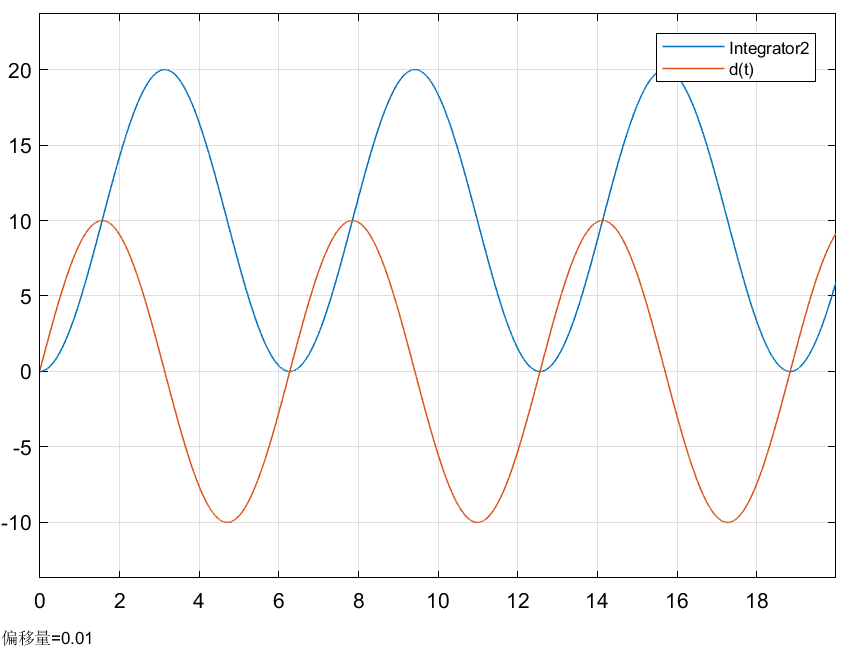
\includegraphics[width=0.25\textwidth]{15.1.jpg}}
    \subfigure[Derivative system]{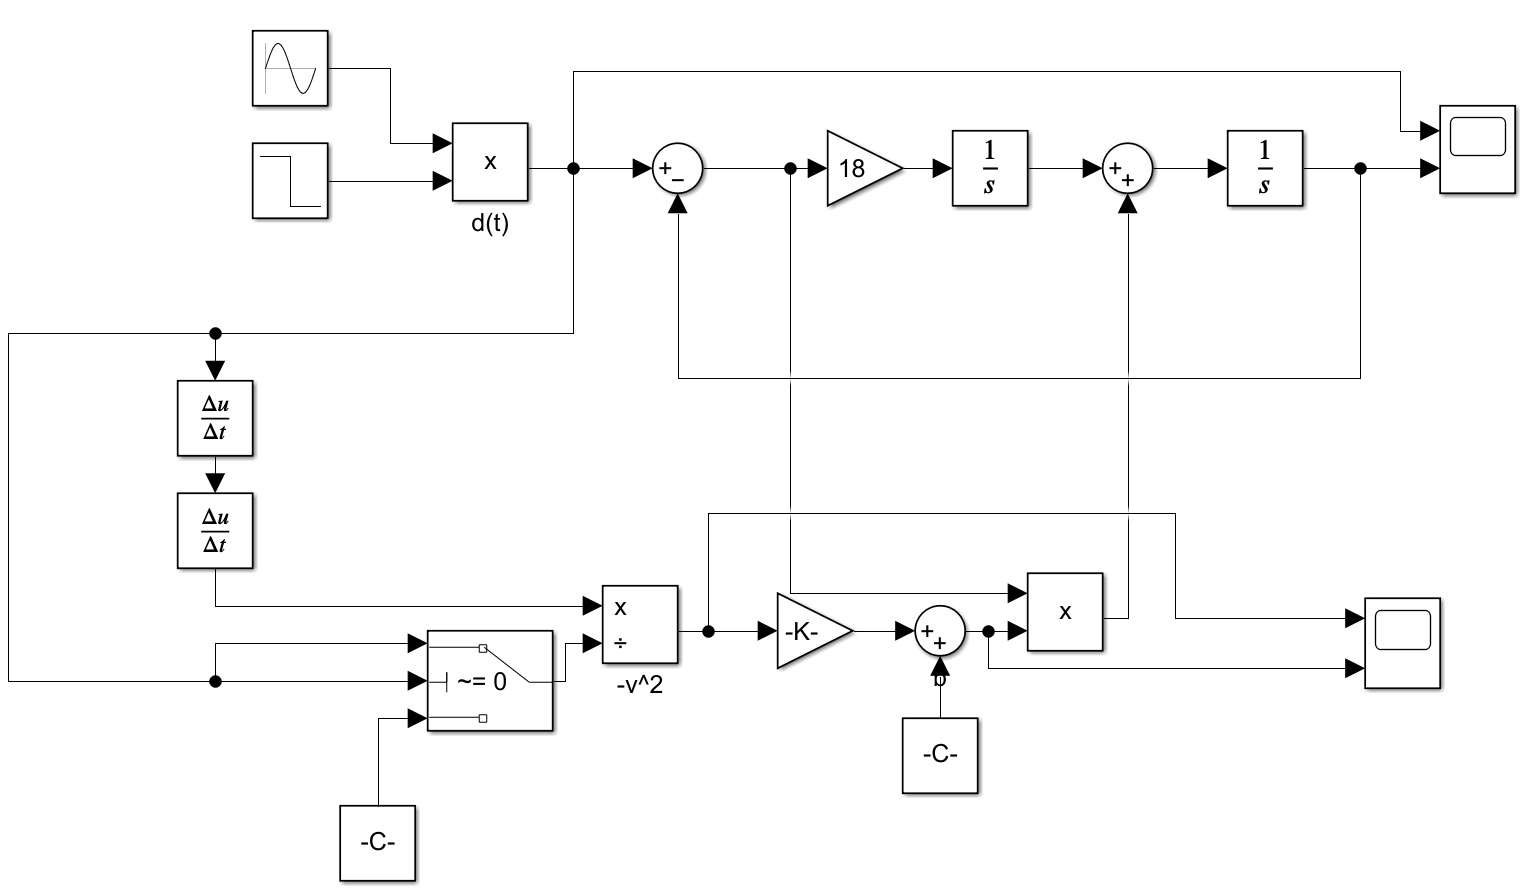
\includegraphics[width=0.35\textwidth]{15.2.png}}
    \subfigure[Derivative for $v=1m/s$]{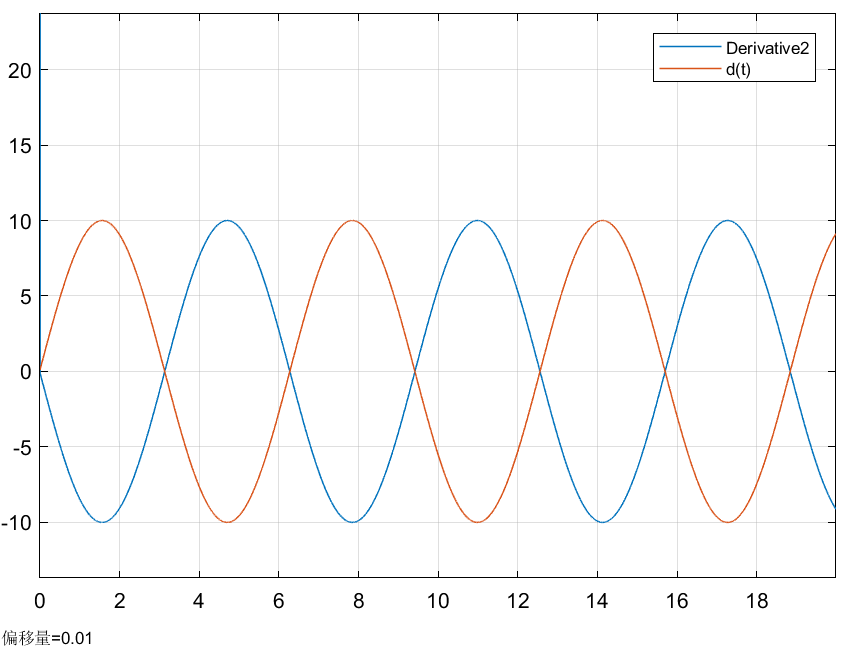
\includegraphics[width=0.25\textwidth]{15.3.jpg}}
    \caption{Observer simulation result}
\end{figure}

If these abnormal values are ignored,
the simulation can be run successfully as shown in figure 16.\\

\begin{figure}[htbp]
    \centering
    \subfigure[Estimated $-v^2$ and corresponding $b$]{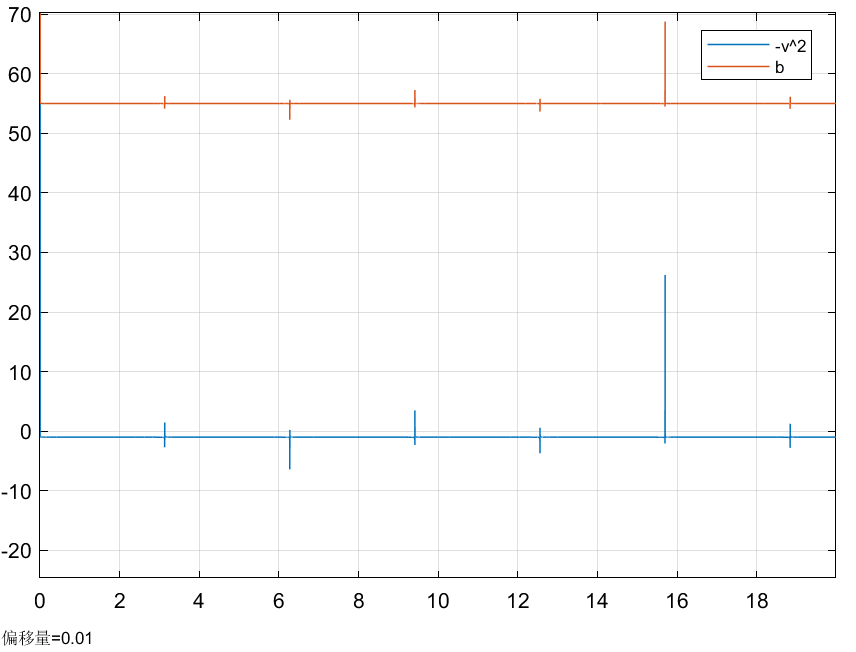
\includegraphics[width=0.3\textwidth]{16.1.jpg}}
    \subfigure[Response of the system]{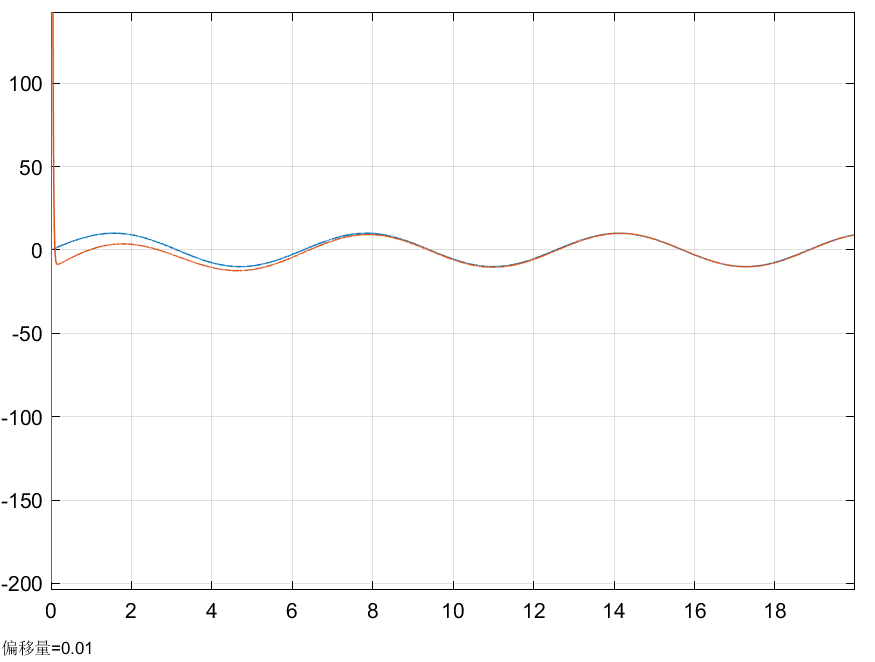
\includegraphics[width=0.3\textwidth]{16.2.jpg}}
    \caption{Observer simulation result for sinusoidal input}
\end{figure}

However, simulation meets another problem when we consider the input signal as transient signal.
This is reasonable since the uneven road surface occur randomly and does not last for a long time.
When the input signal stops, i.e. the input signal is zero,
the estimated speed will be zero as well.
This will lead to an incorrect $b$ especially when $v$ is large,
thus the system will be unstable as shown in figure 17.\\

\begin{figure}[htbp]
    \centering
    \subfigure[Estimated $-v^2$ and corresponding $b$]{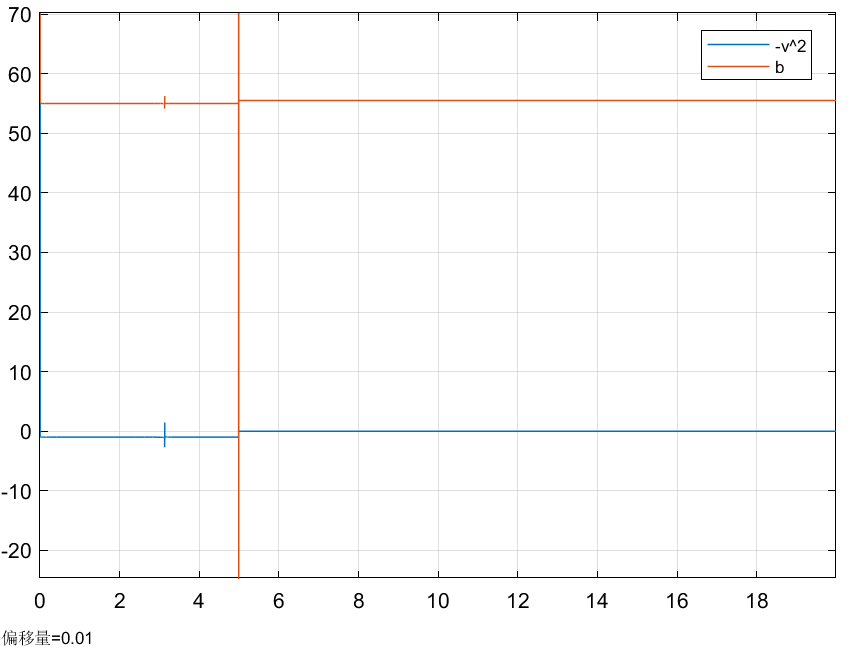
\includegraphics[width=0.3\textwidth]{17.1.jpg}}
    \subfigure[Response of the system]{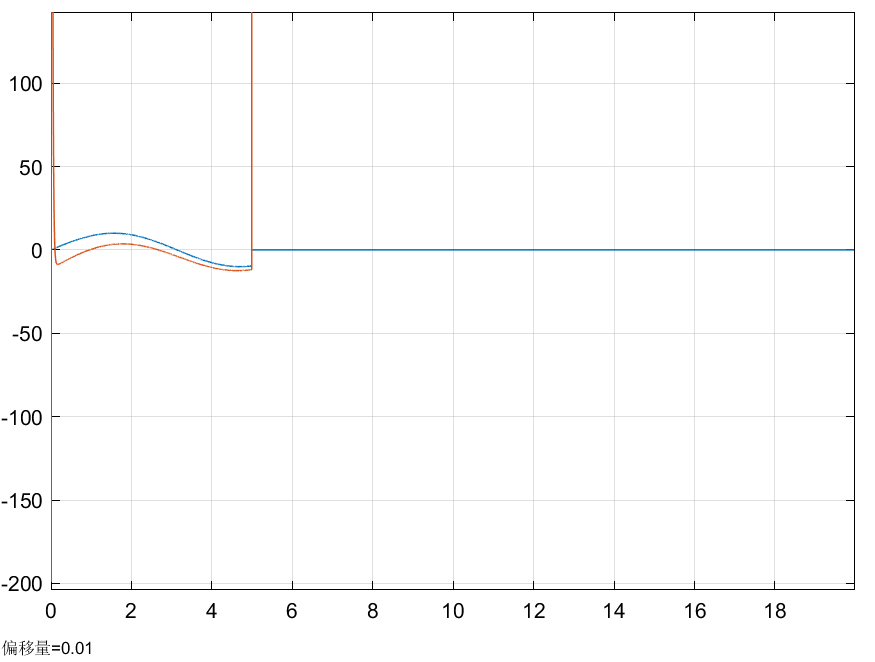
\includegraphics[width=0.3\textwidth]{17.2.jpg}}
    \caption{Observer simulation result for transient input}
\end{figure}

\subsubsubsection{Discussion}

Use the input signal to estimate the speed is only feasible when the input signal is sinusoidal.
However, this assumption is not reasonable in the real world.
Even for a constant speed, the frequency of the input signal will be affected by 
the length of the uneven road surface.
What we interested in is the relationship between the speed and $b$,
not the relationship between the input signal and $b$.
Therefore, it is not necessary to use the input signal to estimate the speed.
Especially, modern cars are equipped with pecise speed sensors,
which can give us a much more accurate speed information.\\

\subsubsection{Digital control law}

Using the linear approximation relationship between $b$ and $v$,
\begin{align*}
    b(v) = \begin{cases}
        5, & v\geq 10\\
        -5v+55, & 0<v<10
    \end{cases}
\end{align*}

Therefore, we can embed the valve position control system into the overall active suspension control system.
First, as the problem tells us that 
the value of $b$ is porportional to the output of the valve position $Y(s)$.
This porportional relationship can be realized by an amplifier easily.
So, we just set the scale factor as $1$ here.\\

\subsection{Simulation result}

As we have discussed in the previous section,
the valve control system has a fast response speed after our analysis.
Therefore, we just build the system in simulink and obtain the following results.\\

\begin{figure}[htbp]
    \centering
    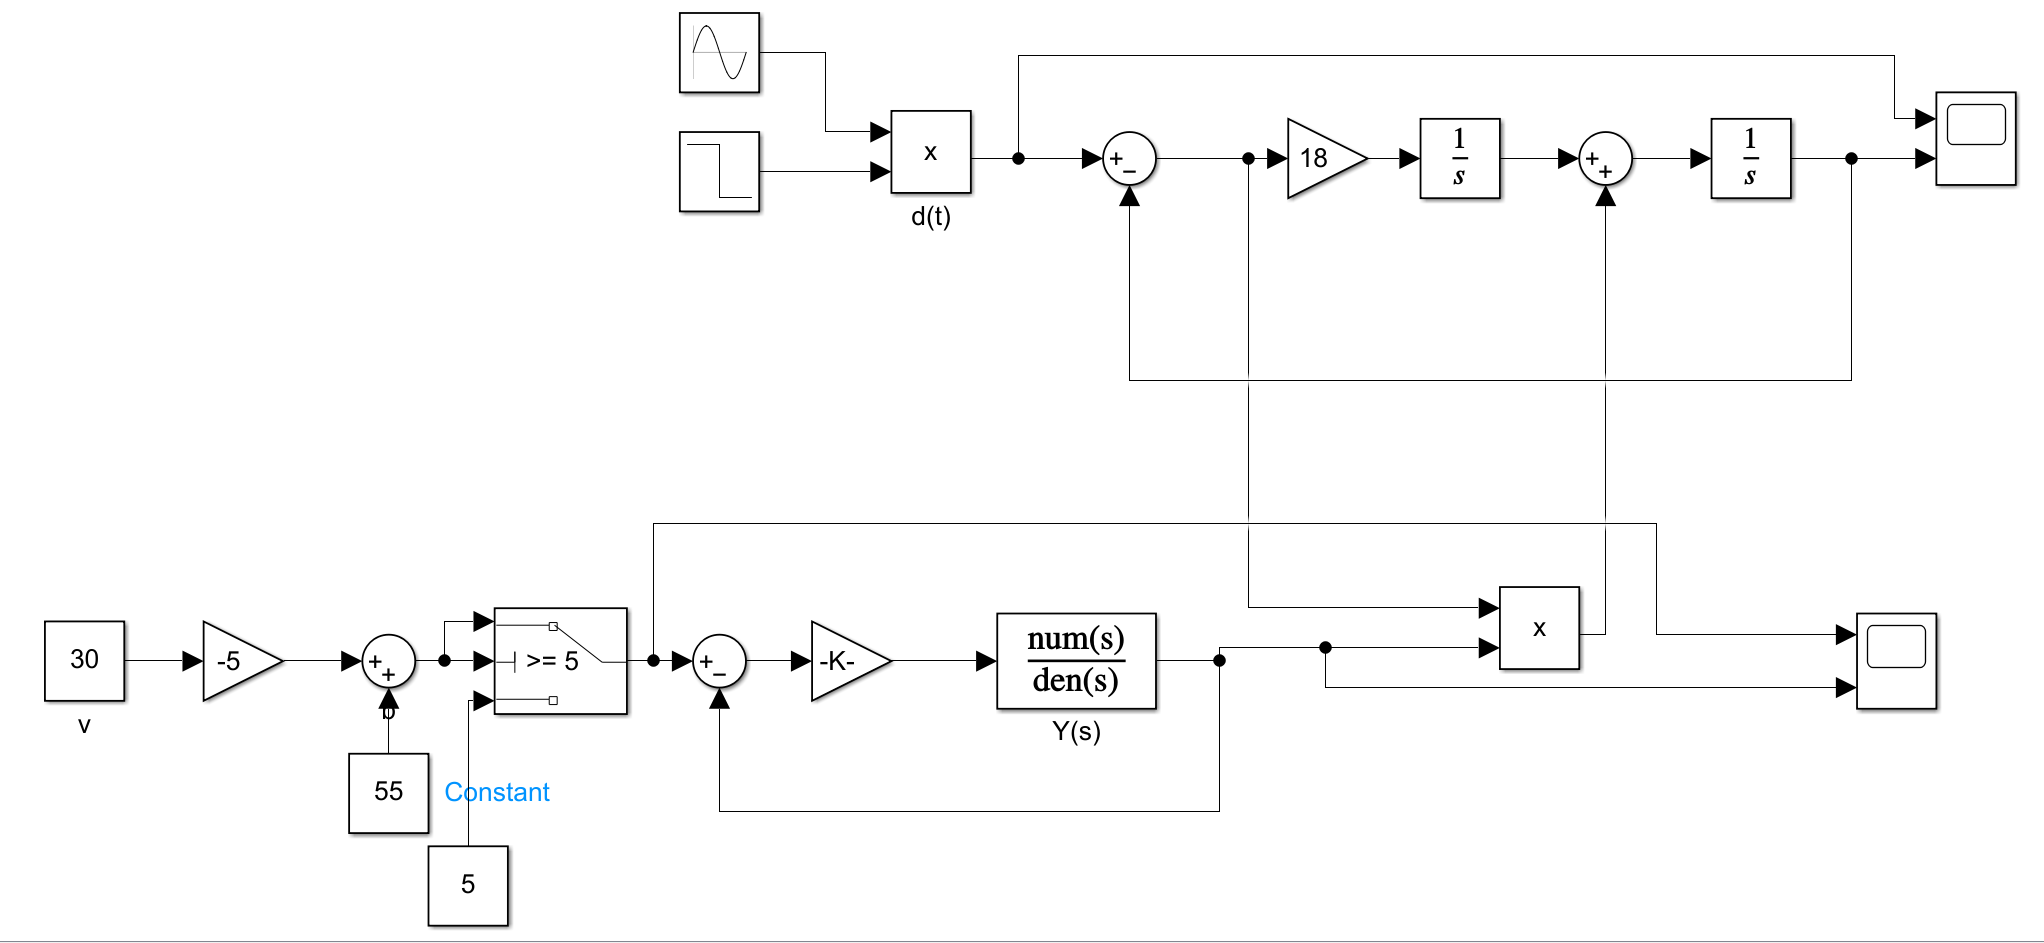
\includegraphics[width=0.7\textwidth]{24.png}
    \caption{Simulink model of the system}
\end{figure}

\begin{figure}[htbp]
    \centering
    \subfigure[Response of the valve]{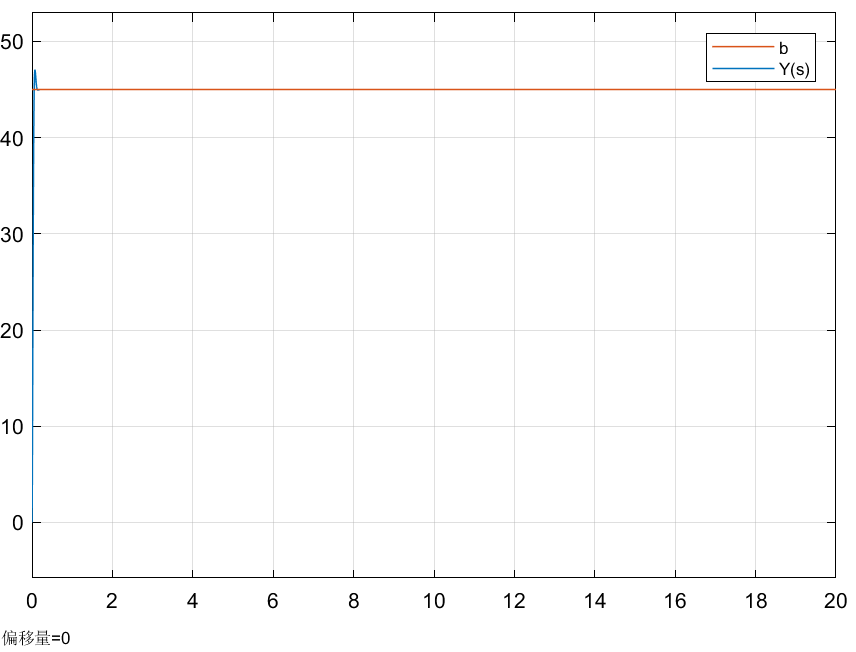
\includegraphics[width=0.4\textwidth]{18.1.jpg}}
    \subfigure[Response of the system]{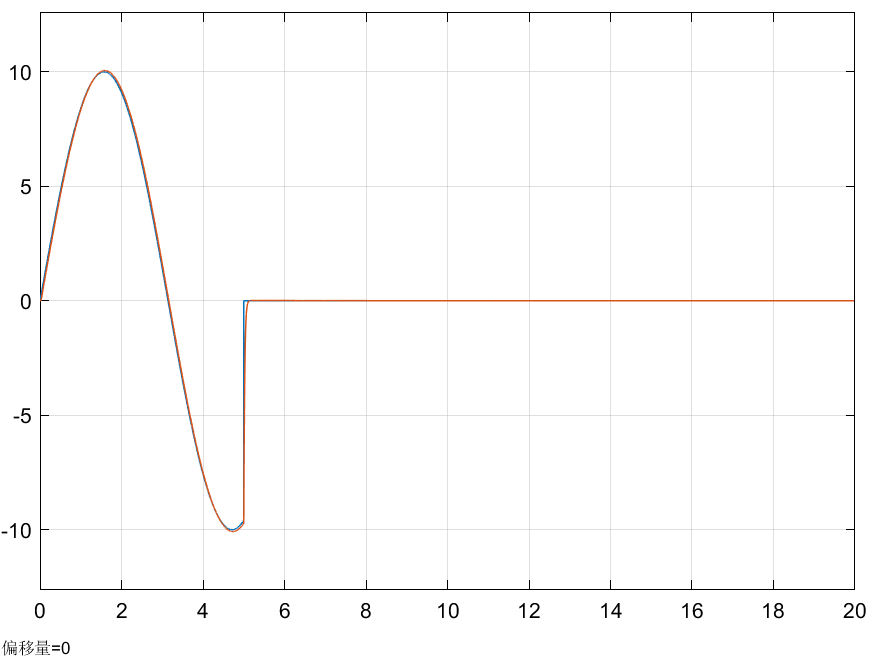
\includegraphics[width=0.4\textwidth]{18.2.jpg}}
    \caption{Simulation result for $v=1m/s$}
\end{figure}

\begin{figure}[htbp]
    \centering
    \subfigure[Response of the valve]{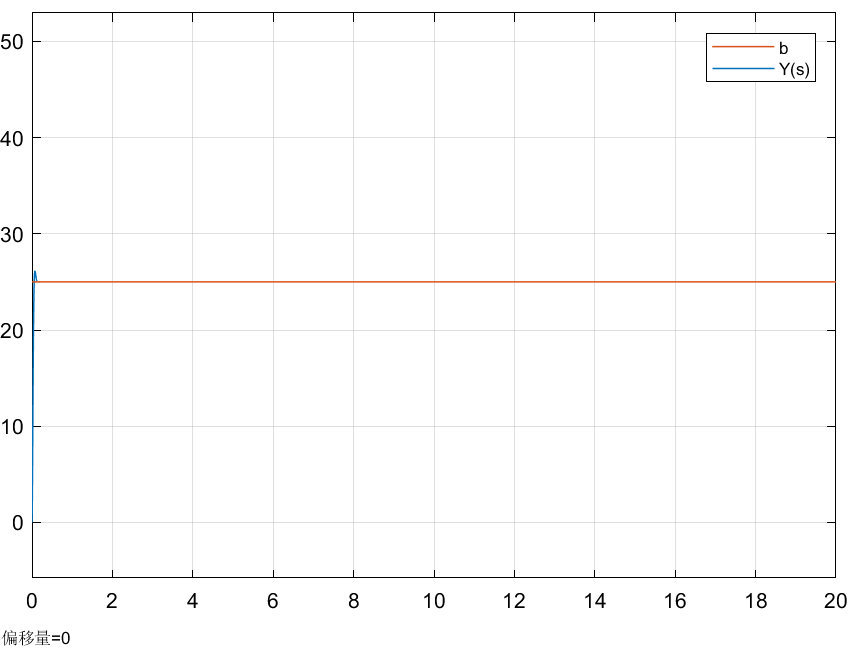
\includegraphics[width=0.4\textwidth]{19.1.jpg}}
    \subfigure[Response of the system]{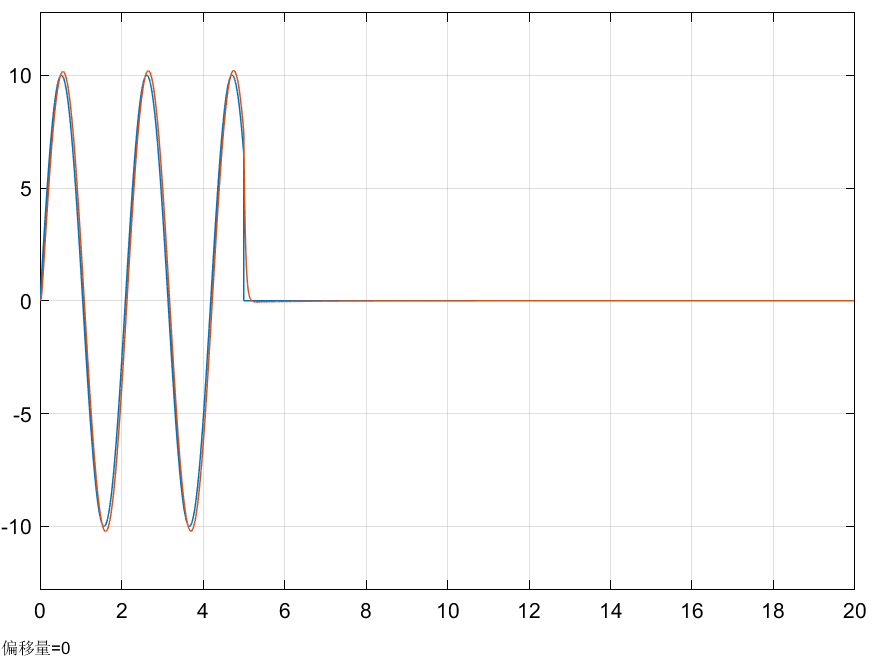
\includegraphics[width=0.4\textwidth]{19.2.jpg}}
    \caption{Simulation result for $v=3m/s$}
\end{figure}

\begin{figure}[htbp]
    \centering
    \subfigure[Response of the valve]{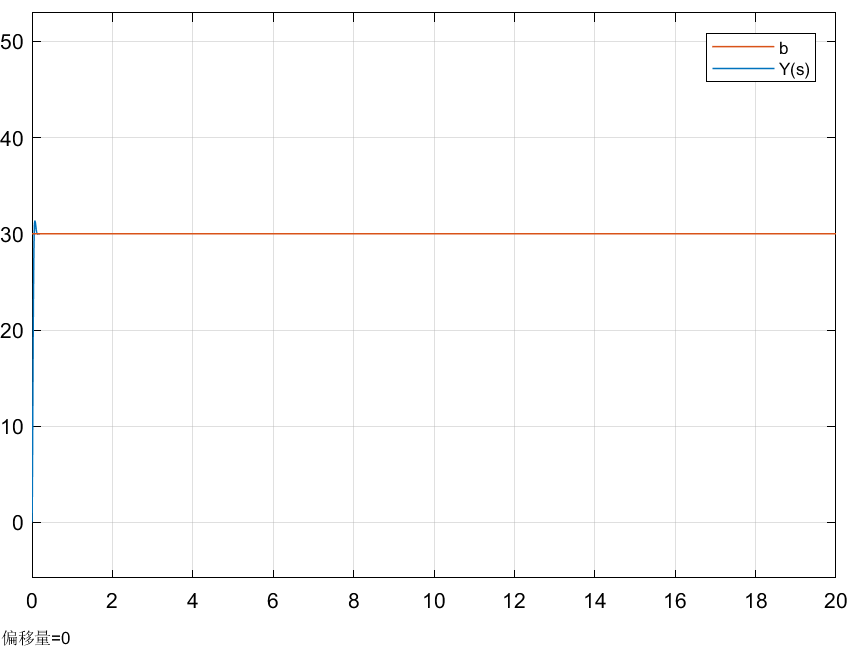
\includegraphics[width=0.4\textwidth]{20.1.jpg}}
    \subfigure[Response of the system]{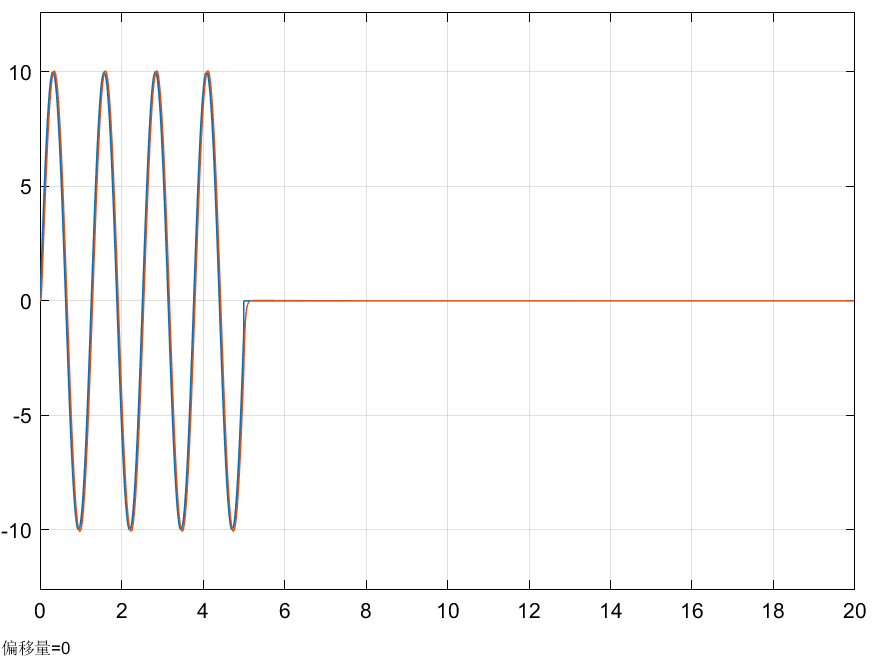
\includegraphics[width=0.4\textwidth]{20.2.jpg}}
    \caption{Simulation result for $v=5m/s$}
\end{figure}

\begin{figure}[htbp]
    \centering
    \subfigure[Response of the valve]{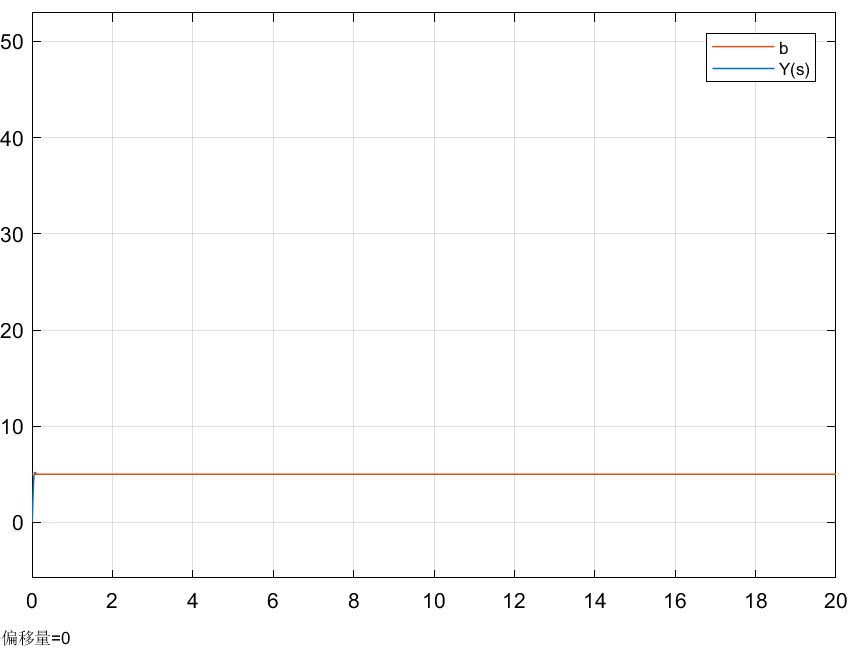
\includegraphics[width=0.4\textwidth]{21.1.jpg}}
    \subfigure[Response of the system]{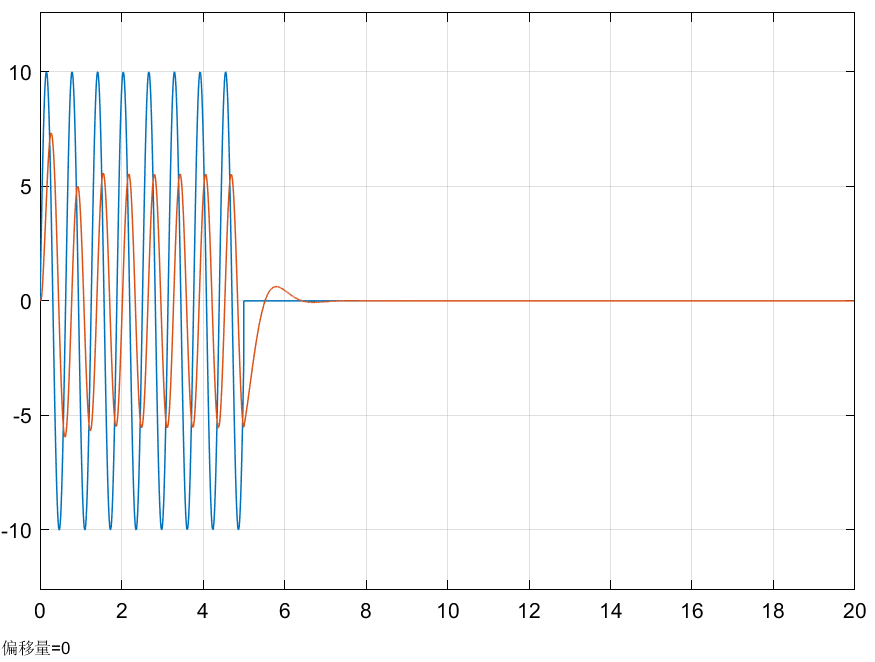
\includegraphics[width=0.4\textwidth]{21.2.jpg}}
    \caption{Simulation result for $v=10m/s$}
\end{figure}

\begin{figure}[htbp]
    \centering
    \subfigure[Response of the valve]{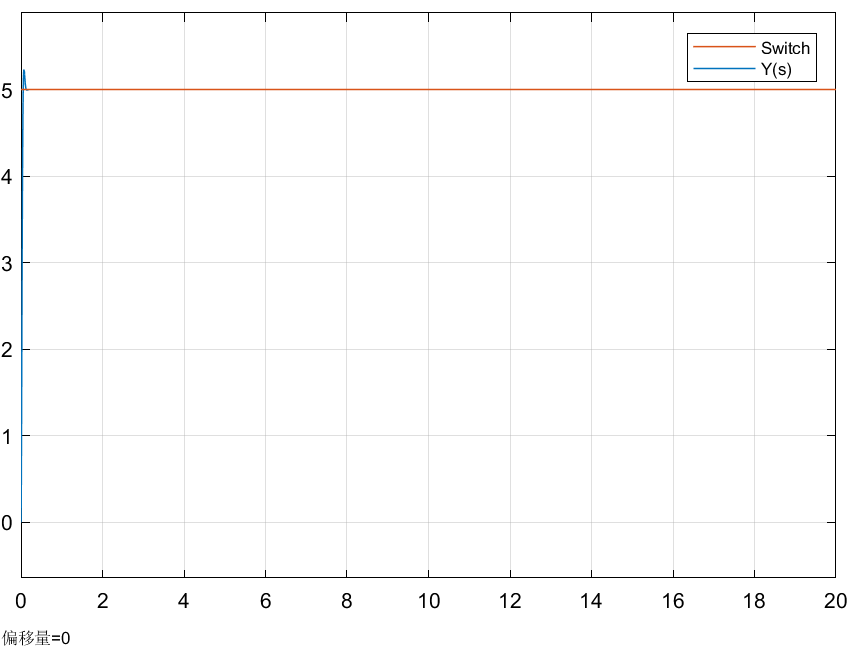
\includegraphics[width=0.4\textwidth]{22.1.jpg}}
    \subfigure[Response of the system]{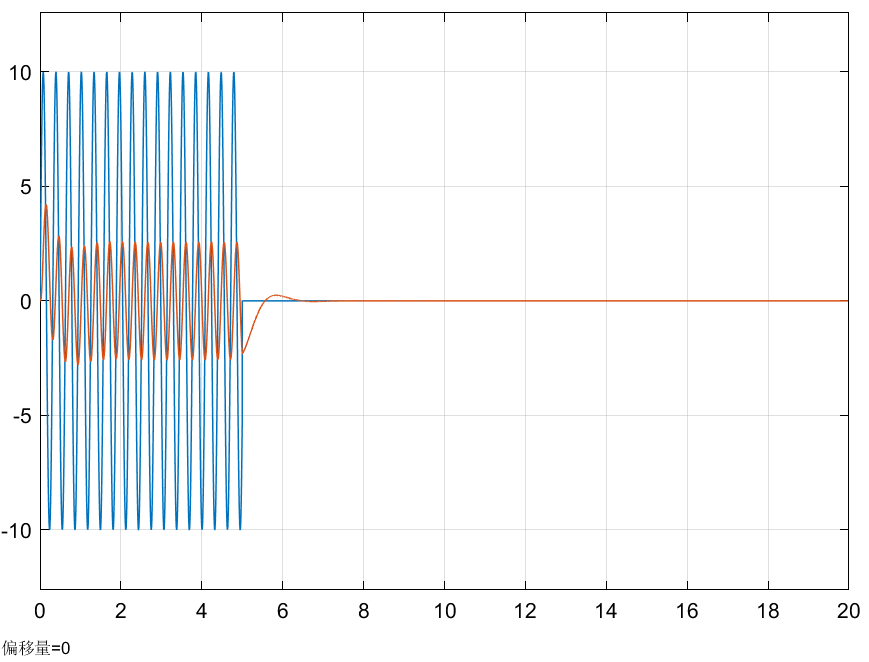
\includegraphics[width=0.4\textwidth]{22.2.jpg}}
    \caption{Simulation result for $v=20m/s$}
\end{figure}

\begin{figure}[htbp]
    \centering
    \subfigure[Response of the valve]{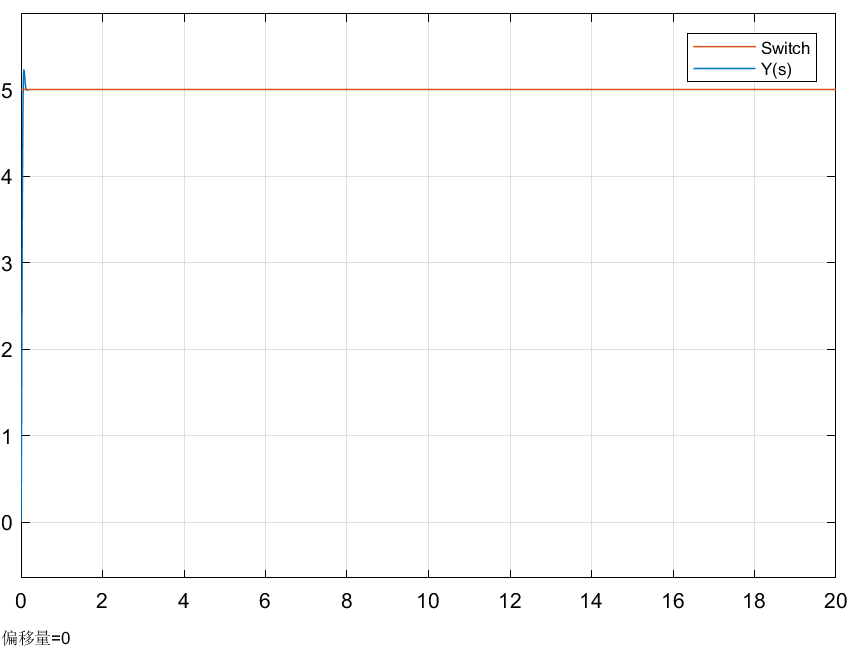
\includegraphics[width=0.4\textwidth]{23.1.jpg}}
    \subfigure[Response of the system]{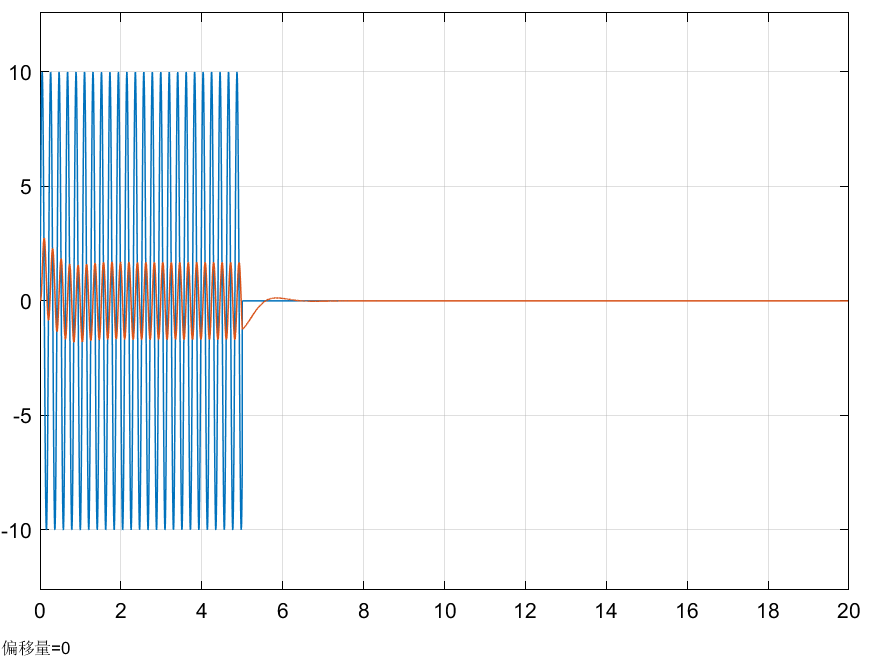
\includegraphics[width=0.4\textwidth]{23.2.jpg}}
    \caption{Simulation result for $v=30m/s$}
\end{figure}

Therefore,
we can see that the system can achieve the desired performance,
i.e. the vehicle accommodates a large bump at high speeds and a small bump at low speeds.
In the other words,
the system won't rise and full with a large amplitude whether it faces 
a large bump at high speed or a small bump at any speed.\\

\section{Conclusion and Discussion}

In this report,
the control law developed for the active suspension system 
has demonstrated its ability to effectively improve ride comfort 
and handling performance of a vehicle. 
Through the use of sensors and actuators, 
the control law is able to continuously monitor 
and adjust the suspension to changing road conditions, 
resulting in a smoother and more stable ride. 
The results of our simulations and experiments show that 
the active suspension system significantly reduces body vibrations,
leading to improved vehicle performance and safety. 
Overall, the implementation of this control law has the potential to 
greatly enhance the driving experience and make it more comfortable and enjoyable 
for the occupants of the vehicle.\\

However,
as we discussed in 3.4.1.2,
we have made such an impractical assumption that
the input signal is a sine wave with a constant frequency.
In the real world,
the frequency of the input signal will be affected by the length of the uneven road surface
and the speed of the vehicle.
Therefore,
a simple linear approximation relationship between $b$ and $v$ is not enough to describe the relationship between $b$ and $v$.
In the future,
we can use a more complex model to describe the relationship between $b$ and $v$.

\section{Division of Labor}

ZhuYuxuan: Simulink, Final report, Presentation\\

DaiLiangtao: Other matlab codes, Initial report, PowerPoint\\

% \section{Time Domain Analysis}
% Before we embed the valve position control system into the overall active suspension control system,
% we need to build the state space model of the suspension system.
% Define the following state variables:
% \begin{align*}
%     z(t)&=\begin{bmatrix}x(t)-d(t)\\ \dot{x}(t)-\dot{d}(t)\end{bmatrix}\\
%     u(t)&=-\ddot{d}(t)
% \end{align*}

% Then, we can get the following state space model:
% \begin{align*}
%     \dot{z}(t) &= \begin{bmatrix}0&1\\-\frac{k}{M}&-\frac{b}{M}\end{bmatrix}z(t)+\begin{bmatrix}0\\ 1\end{bmatrix}u(t)\\
%     y(t) &= \begin{bmatrix}\frac{k}{M}&\frac{b}{M}\end{bmatrix}z(t)
% \end{align*}

% Therefore, to simulate the system,
% we have set the input as $x(t)-d(t)$, the output as $\ddot{x}(t)$.

\begin{thebibliography}{1}
    \bibitem{1} Modern Control Systems, thirteenth edition, Richard C.Dorf, Robert H. Bishop, 2012.
    \bibitem{2} A. Titli, S. Roukieh and E. Dayre, Three control approaches for the design of car semi-active suspension
    (optimal control, variable structure control, fuzzy control), Proceedings of 32nd IEEE Conference on
    Decision and Control, 1993.
    \bibitem{3} Ashley S. Putting a suspension through its paces[J]. Mechanical Engineering-CIME, 1993.
    \bibitem{4} Hrovat D. Applications of optimal control to advanced automotive suspension design[J]. 1993.
\end{thebibliography}


\end{document}
